\documentclass[11pt,a4paper]{article}
\usepackage[left=25mm,right=15mm,top=15mm,bottom=15mm]{geometry}
\usepackage[L7x]{fontenc}
\usepackage[utf8x]{inputenc}
\usepackage[lithuanian]{babel}
\usepackage{./cyrillic}
\usepackage{tikz}
\usepackage{pgfplots}
\usepackage{graphics}
\usepackage{latexsym}
\usepackage{amsmath, amssymb}
\usepackage[europeanresistor]{circuitikz}
%% Crylic fonts
\newcommand{\cyrrm}{\fontencoding{OT2}\selectfont\textcyrup}

\begin{document}
\begin{titlepage}
  
  \begin{center}
    \textsc{\LARGE Vilniaus Gedimino Technikos universitetas}\\[2mm]
    \textsc{\Large Elektroninių sistemų katedra}\\[70mm]
    \textsc{\Large Terminės difuzijos proceso tyrimas, tranzistorių ekvivalentinių grandinių schemų sudarymas ir akustoelektroninio įtaiso projektavimas}\\[10mm]
    \textsc{\normalsize Elektronikos įtaisų kursinio darbo užduotis}\\[40mm]
    \begin{minipage}{1\textwidth}
      \begin{flushright}
        \emph{Darbą atliko:} EI-08/2 gr. studentas\\ Maksim Norkin\\
        \emph{Darbą tikrino:} V.Malinauskas\\
      \end{flushright}
    \end{minipage}
    \vfill
    {\large Vilnius \\ \the\year}
  \end{center}
\end{titlepage}
\tableofcontents
\newpage
\section{Įvadas}

Svarbiausieji šiuolaikinės elektroninės aparatūros komponentai yra silicio integriniai grandynai. Jų elementai 
ir juos jungiantys laidieji takeliai suformuojami vienu technologinių procesų ciklu ir sudaro nedalomą visumą.\\

Silicio integrinių grandynų gamybos technologinius procesus galima suskirstyti į tris grupes:
\begin{itemize}
	\item Silicio plokštelių bei grandynų korpusų detalių ir mazgų gamybos procesai.
	\item Puslaidininkių elementų formavimo silicio plokštelėse procesai.
	\item Integrinių grandynų surinkimo, kontrolės ir bandymo procesai.
\end{itemize}

Analizuojant tranzistorinius stiprintuvus ir kitus įtaisus, tranzistoriai pakeičiami ekvivalentinėmis grandinėmis. 
Viena ar kita ekvivalentinė grandinė pasirenkama, atsižvelgiant į tai, koks klausimas nagrinėjamas.\\

Kai nagrinėjamas tik silpnų virpesių perdavimas, nepaisoma tranzistoriaus įtampų ir srovių nuolatinių dedamųjų. 
Tada tranzistoriaus ekvivalentinės grandinės sudaromos remiantis lygtimis, aprašančiomis tranzistorių kaip tiesinį 
aktyvųjį keturpolį. Dažniausiai naudojamos $T$ ir $\Pi$ pavidalo ekvivalentinės grandinės.\\

Didėjant integrinių grandynų integracijos laipsniui, mažėja elektroninės aparatūros masė, tūris, savikaina, didėja jos patikimumas, 
plečiasi funkcinės galimybės. Kita vertus, integriniuose grandynuose dažniiausiai realizuojami tik tranzistoriai, diodai, rezistoriai 
ir nedidelės talpos kondensatoriai.\\

Nuo tada, kai buvo sukurti integriniai grandynai, iškilo filtrų, vėlinimo linijų ir kitų komponentų, kuriems reikalingi 
induktyvumo elementai, miniatiūrizavimo problema. Sprendžiant šią problemą, buvo tobulinami aktyvieji filtrai, 
komutuojamos talpos filtrai, diegiami skaitmeniniai informacijos apdorojimo būdai. Be to, virpesių 
filtravimui ir vėlinimui buvo pradėtos taikyti paviršinės akustinės bangos, ir susiformavimo nauja funkcinės elektronikos 
kryptis - akustinė elektronika.\\

Kursinio darbo metu ištirsine terminės difuzijos procesą, kuris taikomas antrame silicio integrinių grandynų 
gamybos technologiniam procese, sudarysim tranzistorių ekvivalentinų grandinių schemas ir suprojektuosime akustoelektronikos įtaisą.\\

\section{Šiluminė priemaišų difuzija}
Difuzija ( log. \emph{diffusio} - sklidimas ) yra kryptingas medžiagos dalelių skverbimasis jų tankio mažėjimo 
link dėl šių dalelių chaotiško judėjimo. Gaminant puslaidininkinius įtaisus ir puslaidininkinius integrinius grandynus, 
difuzijos reiškinys panaudojamas puslaidininkiams legiruoti. Aukštoje temperatūroje difuzijos būdu į 
paviršinį puslaidininkio sluoksnį įterpus priemaišų, galima pakeisti šio sluoksnio laidumo tipą arba sudaryti lokaliąsias kitokio laidumo sritis.
\subsection{Priemaišų difuzijos mechanizmas ir greitis}
Šiluminė priemaišų difuzija vyksta dėl difunduojančios medžiagos - difuzanto - koncentracijos gradiento.\\

Priemaišiniai atomai į kietuosius kūnus gali skverbtis keliais būdais: užimdami vakansijas, prasiskverbdami tarp mazgų ir pasikeisdami vietomis su gretimais atomais.\\

Tikimiausias yra pirmasis priemaišų atomų difuzijos mechanizmas, nes aukštoje temperatūroje vakansijų gali būti gana daug. 
Jos atsiranda kaip Šotkio arba Frenkelio defektai. Kylant temperatūrai, vakansijų tankis auga, priemaišinių atomų skverbimosi per 
vakansijas tikimybė didėja. Beje, didėjant prasiskverbusių į padėklą priemaišų tankiui ir dėl to mažėjant vakansijų tankiui, svarbesnis 
tampa antrasis priemaišų skverbimosi kelias - per tarpmazgius. Mažiausiai tikėtinas trečiasis priemaišinių atomų skverbimosi būdas, nes 
gretimi atomai gardelės mazguose gali pasikeisti vietomis tik įgiję gana daug energijos.\\

Difuzijos proceso greitį apibūdina difuzijos koeficientas. Šiluminės priemaišų difuzijos koeficientas $D$ paprastai išreiškiamas 
kvadratiniais centimetrais per sekundę ($cm^2/s$). Jo skaitinę vertę reiškia skaičių dalelių, pereinančių per $1\;cm^2$ plotą 
per $1\;s$, kai priemaišos atomų tankio gradientas lygus $1\;cm^{-4}$.\\

Difuzijos koeficientas labai priklauso nuo temperatūros. Jai kylant, difuzijos koeficientas sparčiai didėja. 
Priklausomybė $D(T)$ išreiškiama Arenijaus ($Arrhenius$) lygtimi:\\

\begin{equation}
  D = D_0 e^{-W_a/kT};
\end{equation}
čia $D_0$ - proporcingumo koeficientas; $W_a$ - difuzijos proceso aktyvacijos energija; $k$ - Bolcmano konstanta; $T$ - difuzijos proceso temperatūra.\\

Koeficientas $D_0$ priklauso nuo puslaidininkio ir priemaišos tipo, kristalo-grafinės krypties, 
kuri vyksta difuzija, ir pradinio priemaišų tankio. Aktyvacijos energija $W_a$ priklauso nuo puslaidininkio, 
priemaišos tipo ir difuzijos mechanizmo. Jei į silicį difunduoja boras, tai $W_a \approx 3,7$ eV, jei fosforas, - 4,4 eV.\\

Kadangi koeficientas $D_0$ ir aktyvacijos energijos energija $W_a$ priklauso nuo daugelio veiksnių, 
tai ankstesnė lygtis gerai tinka tik difuzijos koeficiento $D$ priklausomybių nuo $T$ ir $W_a$ pobūdžiui išreikšti. 
Praktikoje priemaišos difuzijos koeficientas randamas iš literatūroje pateikiamų grafikų, sudarytų remiantis eksperimentų rezultatais.
\subsection{Difuzijos procesų teorija}
Difuzijos teorija pagrįsta dviem dėsniais, kuriuos 1855 m. suformulavo šveicarų mokslininkas A.Fikas (\emph{Fick}).\\

Taikydami pirmą difuzijos dėsnį priemaišų difuzijai ir laikydami, kad priemaišiniai atomai skverbiasi į kristalą $x$ ašies kryptimi, galime rašyti:
\begin{equation} 
  J(x,t) = - D \frac{\delta N(x,t)}{\delta x}
\end{equation}
čia $J$ - priemaišos atomų srauto tankis, $N$ - priemaišos atomų tankis, $t$ - laikas.\\

Antro Fiko dėsnio matematinę ištaišką galima išvesti remiantis pirmuoju dėsniu.\\

Imkime ploną sluoksnį $\delta x$ tarp dviejų vienetinio ploto plokštumų, statmenų difuzinio srauto krypčiai. 
Sakykime, kad priemaišos tankis sluoksnyje laiko momentu $t$ yra $N(x,t)$. Prabėgus laikui $\delta t$, 
priemaišos tankis tampa $N(x,t+ \delta t)$. Tada priemaišos atomų skaičiaus pokytis nagrinėjamame sluoksnyje per laiką $\delta t$ yra
\begin{equation}
[ N (x,t+\delta t ) - N(x,t) ] \delta x = \frac{\delta N(x,t)}{\delta t} \delta t \delta x
\end{equation}
Priemaišos tankis kinta todėl, kad priemaišos atomų srautas $J(x,t)$, tekantis į nagrinėjamąjį sluoksnį per 1 plokštumą, 
skiriasi nuo ištekančio per 2 plokštumą srauto $J(x+\delta x,t)$. Dėl to, kad šie srautai nevienodi, 
priemaišos atomų skaičiaus pokytį sluoksnyje $\delta x$ per elementarųjį laiką $\delta t$ galima išreikšti formule:
\begin{equation}
 [J(x,t) - J(x + \delta x,t ) ] \delta t = - \frac{\delta J(x,t)}{\delta x} \delta x \delta t. 
\end{equation}
Sulyginę ankstesnes dvi formules, gauname:
\begin{equation}
\frac{\delta N(x,t)}{\delta t} = - \frac{\delta J(x,t)}{\delta t} 
\end{equation}
Įrašę į šią lygtį srauto tankio išraišką, gauname diferencialinę lygtį, kuria išreiškiamas antrasis Fiko dėsnis:
\begin{equation}
\frac{\delta N(x,t)}{\delta t} = D \frac{\delta^2 N(x,t)}{\delta x^2} 
\end{equation}
Ši lygtis aprašo primaišos kaupimosi greitį. Ja naudojantis galima nagrinėti difuzijos proceso dinamiką.\\

Išsprendus antro Fiko dėsnio lygti, randama priemaišos tankio priklausomybė nuo difuzijos trukmės ir koordinatės, 
taigi galima apskaičiuoti priemaišos pasiskirstymą kristale bet kuriuo laiko momentu. 
Priemaišos tankio priklausomybė nuo koordinatės vadinama koncentracijos profiliu, arba legiravimo profiliu.\\

Praktikoje pasitaikančias priemaišų difuzijos sąlygas gana greitai atitinka du paprasti teoriniai modeliai: difuzija iš nesenkančio šaltinio ir difuzija iš riboto šaltinio.\\

Laikoma, kad difuzijos šaltinis yra nesenkantis, jeigu priemaišos atomų tankis kristalo paviršiuje nekinta - jeigu $N(0,t) = N_0 = const$, 
kai $t \geq 0$. Atsižvelgus į pradinę sąlygą $N(x,t) = 0$, kai $x \geq 0 $ ir $t=0$, bei ribinę sąlygą $N(x,t)=0$, 
kai $x \rightarrow \infty$ ir $t \geq 0$, gaunamas toks antrosios Fiko diferencialinės lygties sprendinys:
\begin{equation}
N(x,t) = N_0\;erfc\frac{x}{2\sqrt{Dt}}
\end{equation}
čia erfc - papildoma paklaidų funkcija ( \emph{error function complement} ), išreiškiama formule:
\begin{equation}
erfc(y) = 1 - \frac{2}{\sqrt{\pi}} \int^y_0 exp(-y^2) \delta y
\end{equation}
Dydis $\sqrt{Dt}$ vadinamas difuzijos nuotoliu.\\
Pagal $N(x,t)$ išraišką, priemaišos atomų tankio pasiskirstymą lemia difuzijos koeficientas $D$ ( proceso temperatūra T ) ir difuzijos proceso trukmė $t$. Vykstant difuzijai iš nesenkančio šaltinio, didesniame gylyje priemaišos tankis yra mažesnis. Tam tikrame gylyje, kol vyksta difuzija, priemaišos atomų tankis didėja. Jei difuzijos procesas vyktų pakankamai ilgai, priemaišos atomų tankis bet kuriame gylyje taptų toks, kaip paviršiuje.\\

Nuo difuzijos proceso temperatūros ir trukmės priklauso ir legiravimo dozė $Q$ -  skaičius priemaišos atomų, perėjusių per vienetinį padėklo paviršiaus plotą per difuzijos laiką $t$.\\

Žinodami $N(x,t)$, galime rasti difuzijos srauto tankį. Taikydami pirmajį Fiko dėsnį, galime rašyti:
\begin{equation} 
J(0,t) = - D\frac{\delta N(x,t)}{\delta x}|_{x=0}
\end{equation}
Į šią formulę įrašę priemaišos pasiskirstymo išraišką, gauname:
\begin{equation}
J(0,t) = D\frac{N_0}{\sqrt{\pi Dt}} e^{-(x/2\sqrt{Dt})^{2}}|_{x=0} = N_0 \sqrt{\frac{D}{\pi}}
\end{equation}
Suintegravę priemaišos atomų srautą per vienetinio ploto padėklo paviršių, gauname legiravimo dozę:
\begin{equation}
Q(t) = \int^{t}_{0}J(0,t)\delta t = ... = 2N_0 \sqrt{\frac{Dt}{\pi}} 
\end{equation}
Praktikoje šiluminės priemaišų difuzijos procesą dažniausiai sudaro dvi stadijas. Difuzija iš nesenkančio šaltinio vyksta pirmojoje - \emph{priemaišų įterpimo} stadijoje. Šioje stadijoje į ploną paviršinį kristalo sluoksnį įterpiamas reikiamas priemaišos kiekis. Antrojoje - \emph{priemaišų perskirstymo} stadijoje - aukštesnėje temperatūroje suformuojamas legiravimo profilis.\\

Dažnai antrojoje difuzijos stadijoje atliekamas ir paviršiaus oksidavimas. Todėl antrojoje stadijoje priemaišiniai atomai per padėklo paviršių neprasiskverbia ir legiravimo dozė nekinta. Tada difuzija vyksta iš riboto šaltinio - iš pirmojoje stadijoje legiruoto paviršinio sluoksnio. Šiomis sąlygomis antrosios Fiko diferencialinės lygties sprendinys išreiškiamas formule:
\begin{equation}
N(x,t') = \frac{Q}{\sqrt{\pi D't'}} exp \left (-\frac{x^2}{4D't'} \right ) 
\end{equation}
čia $D'$ - priemaišos difuzijos koeficientas priemaišų perskirstymo etape, t' - šio etapo trukmė.\\

Pastaroji formulė atitinka Gauso ( Gauss ), arba normalųjį, pasiskirstymą. Kreivių parametras yra difuzijos koeficiento ir proceso trukmės sandauga. Pradžioje ( kai $D't' = 0$ ) priemaišos atomų tankis padėklo paviršiuje paprastai atitinka ribinį priemaišos tirpumą. Didėjant sandaugai $D't'$, priemaišiniai atomai iš paviršinio sluoksnio skverbiasi gilyn į padėklą. Todėl prie padėklo paviršiaus priemaišos tankis mažėja, padėklo gilumoje - didėja. Kreivių ribojamas plotas nekinta, nes nekinta legiravimo dozė.\\

Remiantis gautomis išraiškomis, galima teoriškai parinkti šiluminės priemaišų difuzijos procesų sąlygas.\\

Sakykime, kad į padėklą, kuriame pradinis priemaišos atomų tanki $N_{pr}$, atliekama kito tipo priemaišos šiluminė difuzija. Po antrosios difuzijos stadijos padėklo paviršiuje reikia gauti difunduojančios priemaišos atomų tankį
 $N_0$. Kito laidumo tipo difuzinio sluoksnio storis (pn sandūros gylis) turi būti $x_{pn}$.\\
 
Pagal suformuluotą užduotį turi būti tenkinamos sąlygos $N(0,t) = N_0$ ir $N(x_{pn},t) = N_{pr}$. Pasinaudoję šiomis sąlygomis, gauname:
\begin{equation}
N_0 = \frac{Q}{\sqrt{\pi D't'}}
\end{equation}
ir
\begin{equation}
N_{pr} = \frac{Q}{\sqrt{\pi D't'}}exp \left ( - \frac{x^2_{pn}}{4D't'} \right ) = N_0 exp \left ( - \frac{x^2_{pn}}{4D't'} \right ) 
\end{equation}
Pagal šią išraišką, gauname:
\begin{equation}
x^2_{pn} = 4D't'ln \frac{N_0}{N_{pr}}
\end{equation}
Taikydami šią formulę, galime rasti pn sandūros gylį arba parinkti difuzijos proceso sąlygas ( proceso temperatūrą ir trukmę ), kad sandūra sudarytų reikiamame gylyje. Tuomet, remiantis $N_0$ išraišką, galima rasti legiravimo dozę:
\begin{equation}
Q = N_{0}\sqrt{\pi D't'}
\end{equation}
Žinodami reikalingą legiravimo dozę, pirmosios difuzijos stadijos sąlygas (temperatūrą ir trukmę) galime parinkti remiantis
\begin{equation}
Q(t) = .. = 2N_0 \sqrt{\frac{Dt}{\pi}}
\end{equation}
Panašiai difuzijos proceso režimą teoriškai galima parinkti ir tuo atveju, kai taikoma tik viena - priemaišų įterpimo - stadija. Tuomet reikia remtis
\begin{equation}
N(x,t) = N_0 erfc\frac{x}{2 \sqrt{Dt}}
\end{equation}


\section{Difuzijos proceso tyrimas}
\subsection{Apskaičiuoti ir nubraižyti priemaišų pasiskirstymą po priemaišų įterpimo etapo}
Pradiniai duomenys:\\
Difuzijos koeficienas ($cm^2/s$): $D = 1.8*10^{-13}$\\
Proceso trukmės: $t_1 = 13min = 780s, t_2 = 18min = 1080s$ ir $t_3 = 22min = 1320s$.\\

Difuzija iš nesenkančio šaltinio vyksta pirmojoje - priemaišų įterpimo stadijoje. Jos pasisskirstymas randamas, pasitelkus:
\begin{equation}
N(x,t) = N_0*erfc \left( \frac{x}{x\sqrt{Dt}} \right) 
\end{equation} \\
\begin{tikzpicture}[domain=0:0.005]
  \begin{axis} [
      scale only axis,
      width=400pt,
      height=150pt,
      xlabel={$x$},
      ylabel={$N(x)/N_0$},
      grid=major]
    \addplot[smooth, mark=*] plot function {erfc(x/(2*sqrt(1.8*10**(-13)*780)))};
    \addlegendentry{$t_1$}
    \addplot[smooth, mark=o] plot function {erfc(x/(2*sqrt(1.8*10**(-13)*1080)))};
    \addlegendentry{$t_2$}
    \addplot[smooth, mark=x] plot function {erfc(x/(2*sqrt(1.8*10**(-13)*1320)))};
    \addlegendentry{$t_3$}
  \end{axis}
\end{tikzpicture}\\
\textsl{ 3.1 pav. Priemaišų pasiskirstymas po priemaišų įterpimo etapo.}\\

\subsection{Apskaičiuoti ir nubraižyti, kaip priemaišų įterpimo etape kinta priemaišos srauto tankis ir legiravimo dozė}
Pradiniai duomenys:\\
Priemaišų koncentracija bandinio paviršiuje ($1/cm^2$): $N_0 = 3*10^{20}$\\
Priemaišos srauto tankis išreiškiamas:\\
\begin{equation}
J(0,t) = N_0*\sqrt{\frac{D}{\pi t}}
\end{equation}
\begin{tikzpicture}[domain=0:1]
  \begin{axis} [
      scale only axis,
      width=400pt,
      height=150pt,
      xlabel=$t$,
      ylabel={$J(0, t)$},
      grid=major
    ]
    \addplot[smooth] plot function {3*10**(20)*sqrt(1.8*10**(-13)/(3.14*x))};
  \end{axis}
\end{tikzpicture} \\
\textsl{3.2 pav. Priemaišos srauto tankio pokytis, priemaišų įterpimo etape.}\\

Legiravimo dozė išreiškiama:\\
\begin{equation}
Q(t) = 2*N_0*\sqrt{\frac{Dt}{\pi}}
\end{equation}
\begin{tikzpicture}[domain=0:1]
  \begin{axis} [
      scale only axis,
      width=400pt,
      height=150pt,
      xlabel=$t$,
      ylabel=$Q(t)$,
      grid=major
    ]
    \addplot[smooth] plot function {3*10**(20)*sqrt((1.8*10**(-13)*x)/(3.14))};
  \end{axis}
\end{tikzpicture} \\
\textsl{3.3 pav. Legiravimo dozės pokytis, priemaišų įterpimo etape.}
\subsection{Apskaičiuoti ir nubraižyti priemaišų pasiskirstymą po priemaišų perskirstymo etapo}
Pradiniai duomenys:\\
Legiravimo dozė ($1/cm^3$): $Q = 1.4*10^{13}$;\\
Difuzijos koeficientas ($cm^2/S$): $D = 1.8*10^{-13}$;\\
Proceso trukmės: $t_1 = 81min = 4860s$; $t_2 = 70min = 4200s$; $t_3 = 21min = 1260s$;\\
Priemaišų perskirstymo stadiją galime apibrėžti:\\
\begin{equation}
N(x,t') = \frac{Q}{\sqrt{\pi D' t'}} exp \left( - \frac{x^2}{4D't'} \right)
\end{equation}

\begin{tikzpicture}[domain=0:0.009]
  \begin{axis} [
      scale only axis,
      ylabel=$N(x)$,
      width=400pt,
      height=150pt,
      xlabel=$x$,
      grid=major,
    ]
    % Q/sqrt(pi*D'*t')*exp(-(x^2)/(4*D't'))
    \addplot[smooth,mark=*] plot gnuplot { (1.4*10**(13)/(sqrt(pi*1.8*10**(-13)))*exp(-(x**2)/(4*1.8*10**(-13)*4860))) };
    \addlegendentry{$t_1$}
    \addplot[smooth,mark=o] plot gnuplot { (1.4*10**(13)/(sqrt(pi*1.8*10**(-13)))*exp(-(x**2)/(4*1.8*10**(-13)*4200))) };
    \addlegendentry{$t_2$}
    \addplot[smooth,mark=x] plot gnuplot { (1.4*10**(13)/(sqrt(pi*1.8*10**(-13)))*exp(-(x**2)/(4*1.8*10**(-13)*1260))) };
    \addlegendentry{$t_3$}
  \end{axis}
\end{tikzpicture}\\
\textsl{3.4 pav.  Priemaišų pasiskirstymas po priemaišų perskirstymo etapo.}

\subsection{Apskaičiuoti ir nubraižyti priemaišų pasiskirstymą tranzistoriuje, formuojamame dvikartės difuzijos būdu}

\textsl{3.1 lentelė. Priemaišų formavimo dvikartės difuzijos būdu duomenys.}\\
\begin{tabular}{|r|c|c|c|}\hline
  & Įterpimo stadija & Perskirstymo stadija & Įterpimo stadija \\ \hline
  Priemaišų koncentracija ($1/cm^3$): & $2.5*10^{19}$   & -              & $1.4*10^{21}$ \\ \hline
  Normali temperatūra ($^{\circ}C$):   & $1000$         & $1000$         & $1000$ \\ \hline
  Aktyvacijos energija ($eV$):        & $2.2$          & $3.7$          & $2.9$ \\ \hline
  Difuzijos koeficientas ($cm^2/s$):  & $1.9*10^{-13}$  & $1.4*10^{-13}$  & $3.8*10^{-13}$ \\  \hline
  Stadijos trukmė ($min.$):           & $24$           & $77$           & $42$ \\ \hline
  Faktinė temperatūra ($^{\circ}C$):   & $942$          & $1056$         & $318$ \\ \hline
\end{tabular}\\\\\\
% Dvikartė difuzija
% Bazes difuzija
\begin{tikzpicture}
  \begin{semilogyaxis} [
      scale only axis,
      width=400pt,
      domain=-1:1,
      height=150pt,
      ylabel={$log10(N_D-N_A), 1/cm^3$},
      xlabel={$x, mkm$},
      grid=major
    ]
		%TODO
		\addplot[smooth] file {dvitakte_difuzija.plt};
		
  \end{semilogyaxis}
\end{tikzpicture}\\

\textsl{3.5 pav. Priemaišų pasiskirstymas tranzistoriuje, formuojame dvikartės difuzijos būdu.}

\section{Dvipolio tranzistoriaus parametrų skaičiavimas ir ekvivalentinės grandinės schemos sudarymas}
Pradiniai duomenys:\\
Tranzistorius įjungtas pagal bendro emiterio schemą\\
$I_B = 0.14 mA$, $U_{CE} = 8V$, $f_{T} = 0.9 GHz$;\\
\subsection{Rasti dvipolio tranzistoriaus $h$ parametrus}
Randame tranzistoriaus įėjimo varžą:
\begin{equation}
h_{11E} = \frac{\underline{U}_1}{\underline{I}_1}|_{\underline{U_2} = 0}
= \frac{\Delta U_{BE}}{\Delta I_B}| _{U_{KE} = const = U_{KEQ}}
\end{equation}
\[
h_{11E} = \frac{0.162-0.147}{0.16*10^{-3}-0.14*10^{-3}} = \frac{0.015}{0.02*10^{-3}} = 750 \Omega
\]\\
Randame grįžtamojo ryšio koeficientą:
\begin{equation}
h_{12E} = \frac{\underline{U}_1}{\underline{U}_2}|_{\underline{I_{1}} = 0} = \frac{\Delta U_{BE}}{\Delta U_{KE}}|_{I_{B} = const} = \frac{\Delta U_{BE}}{U_{KE3} - U_{KE1}} |_{I_B = I_{BQ}}
\end{equation}
\[
h_{12E} = \frac{0.162-0.141}{12-4} = \frac{0.021}{8} = 2.6*10^{-3}
\]\\
Randame srovės perdavimo koeficientą:
\begin{equation}
h_{21E} = \frac{\underline{I}_2}{\underline{I}_1} |_{\underline{U_{2}} = 0} = 
\frac{\Delta I_{K}}{\Delta I_{B}} |_{U_{KE} = const} = 
\frac{I_{K3} - I_{K1}}{I_{B3} - I_{B1}} |_{U_{KE} = U_{KEQ}}
\end{equation}
\[
h_{21E} = \frac{23*10^{-3}-10.5*10^{-3}}{0.18*10^{-3}-0.1*10^{-3}} = \frac{14.5*10^{-3}}{0.08*10^{-3}} = 181.25
\]\\
Randame išėjimo laidumą:
\begin{equation}
h_{22E} = \frac{\underline{I}_2}{\underline{U}_2} |_{\underline{I_1} = 0} = \frac{\Delta I_K}{\Delta U_{KE}} |_{I_B = const = I_{BQ}}
\end{equation}
\[
h_{22E} = \frac{15.9*10^{-3}-16.1*10^{-3}}{14-12} = \frac{0.2*10^{-3}}{2} = 0.1*10^{-3} S = 0.1 mS;
\]

\subsection{Sudaryti tranzistoriaus $\Pi$ pavidalo ekvivalentinės grandinės schemą, rasti jos elementų parametrus}

\begin{center}
  \begin{circuitikz}
    % X,Y
    \draw (0,2) to[R, l=$r_B^*$, *-*] (2,2);
    \draw (4,0) to[R, l=$r_{\pi}$, *-*] (4,2);
    \draw (6,0) to[C, l=$C_{\pi}$, *-*] (6,2);
    \draw (6,2) to[C, l=$C_{\mu}$] (8,2);
    \draw (9,0) to[european current source, *-*] (9,2);
    \draw (9,2) node[anchor=south] {$g_mU_{\pi}$};
    \draw (11,0) to[R, l=$r_{0}$, *-*] (11,2);
    % vires
    \draw (0,0) to[short, *-*] (2,0);
    \draw (2,0) to[short] (12,0);
    \draw (2,2) to[short, i=$\underline{I}_1$] (4,2);
    \draw (4,2) to[short] (6,2);
    \draw (8,2) to[short] (11,2);
    \draw (12,2) to[short, *-, i_=$\underline{I}_2$] (11,2);
    \draw (2,0) to[open, v^<=$\underline{U}_{\pi}$] (2,2);
    \draw (0,0) to[open,v^<=$\underline{U}_1$] (0,2);
    \draw (12,2) to[open,v^>=$\underline{U}_2$] (12,0);
    % nodes
    \draw (0,2) node[anchor=east] {$B$};
    \draw (12,2) node[anchor=west] {$K$};
    \draw (6,0) node[anchor=north] {$E$};
    %  \draw (1,-1) to[R, l=$r_E$] (1,-1);
    %  \draw (0,0) to[R, l=$R_1$] (3,0);
  \end{circuitikz}\\
\end{center}
\textsl{4.1 pav. $\Pi$ pavidalo ekvivalentinė grandinė.}\\[5pt]
Randame $\Pi$ pavidalo grandinės ekvivalentinius parametrus\\
Apskaičiuojame tranzistoriaus perdavimo charakteristikos statumą $g_m$, kai $I_{KQ} = 16.1 mA$:\\
\begin{equation}
g_m = 40 * I_{KQ}; 
\end{equation}
\[
g_m = 40 * 16.1*10^{-3} = 0.644;
\]
Apskaičiuojame varžą $r_{\pi}$, $\beta = h_{12E} = 181.25$:
\begin{equation}
  r_{\pi} \cong \frac {\beta}{g_m};\;\;
\end{equation}
\[
r_{\pi} \cong \frac {181.25}{0.644} = 281.4 \Omega;
\]
Apskaičiuojame varžą $r_0$:
\begin{equation}
  r_0 = \frac {100}{I_{KQ}};
\end{equation}
\[
r_0 = \frac {100}{16.1*10^{-3}} = 6211.18 \cong 6.2 k \Omega;
\]
Apskaičiuojame varžą $r_B^*$:
\begin{equation}
  r_B^* = h_{11E} - r_{\pi} = 750 - 281.4 = 468.6 \Omega;
\end{equation}
Apskaičiuosime talpą $C_{\pi}$, kai dažnis $f_T = 0.9 GHz$:
\begin{equation}
  C_{\pi} = \frac{g_m}{2\pi f_T} - C_{\mu};
\end{equation}
\[
C_{\pi} = \frac{0.644}{2 * 3.14 * 0.9*10^{9}} - C_{\mu} = 1.14*10^{-11} - C_{\mu} \;F;
\]

\subsection{Apskaičiuoti išėjimo srovės kintamąją dedamąją, kai kintamoji įėjimo įtampa yra 115mV}
Kintamoji įėjimo įtampa:
\[
\underline{U}_{BE} = 115mV;
\]
Išėjimo srovės kintamąji dedamoji grandinėje yra lygti srovės šaltiniui atstojamojoje grandinėje, todėl:
\begin{equation}
	\underline{I}_{K} = g_m \underline{U}_{\pi};
\end{equation}
$U_{\pi}$ galime rasti
\begin{equation}
	U_{\pi} = \frac{r_{\pi}}{r_{\pi}+r_{B}^*} * \underline{U}_{BE} = \frac{r_{\pi}}{h_{11E}} * \underline{U}_{BE};
\end{equation}
Tuomet ankstesnį reiškinį galime pertvarkyti taip:
\[
	\underline{I}_{K} = g_m \frac{r_{\pi}}{h_{11E}} * \underline{U}_{BE};
\]
Apskaičiuojame:
\[
	\underline{I}_{K} = 0.644 * \frac{281.4}{750} * 115*10^{-3} = 27.8 mA;
\]

\subsection{Rasti žemo dažnio įtampos stiprinimo koeficientą, kai apkrovos varža lygi 892 $\Omega$ }
Apkrovos varža:
\[R_a = 892 \Omega\]
Įtampos stiprinimo koeficientą randame iš tokios formulės:
\begin{equation}
	K_U = \frac{\beta * R_a}{h_{11E}} = \frac{h_{21E} * R_a}{h_{11E}};
\end{equation}
Apskaičiuojame:
\[
	K_U = \frac{ 181.25 * 892 }{750} = 215.57
\]
\section{Lauko tranzistoriaus parametrų skaičiavimas ir ekvivalentinės grandinės schemos sudarymas}

Dranzistoriaus darbo taškas $U_{UI} = 0.5 V$, $U_{SI} = 5 V$.

\subsection{Nubraižyti lauko tranzistoriaus perdavimo charkteristikas, kai $U_{DS} = 3,7,11 V$}

\begin{circuitikz}
  \begin{axis} [
      scale only axis,
      width=400pt,
      height=150pt,
      ylabel={$I_{S}, mA$},
      xlabel={$U_{UI}, V$},
      grid=major,
      legend style={anchor=south west},
    ]
    % 3V
    \addplot [smooth, mark=x] plot coordinates {
      (-2,0.7)
      (-1.5,3.2)
      (-1,6.8)
      (-0.5,10.7)
      (0,15.7)
    };
    \addlegendentry{$U_{SI} = 3V$}
    % 7V
    \addplot [smooth, mark=o] plot coordinates {
      (-2,0.7)
      (-1.5,3.3)
      (-1,6.85)
      (-0.5,11.1)
      (0,16.2)
    };
    \addlegendentry{$U_{SI} = 7V$}
    % 11V
    \addplot [smooth, mark=*] plot coordinates {
      (-2,0.7)
      (-1.5,3.4)
      (-1,7)
      (-0.5,11.4)
      (0,16.8)
    };
    \addlegendentry{$U_{SI} = 11V$}
  \end{axis}
\end{circuitikz}\\
\textsl{5.1 pav. Lauko tranzistoriaus perdavimo charakteristikos, kai $U_{SI} = 3V,\;7V,\;11V$.}
  
 
\subsection{Apskaičiuoti lauko tranzistoriaus parametrus nurodytame darbo taške}

Tranzistoriaus perdavimo charakteristikos statumą nurodytame darbo taške, randame:
\begin{equation}
  g_m = S = \frac{\delta I_S}{\delta U_{UI}}
\end{equation}
\[
g_m = S = \frac{16*10^{-3}-6.8*10^{-3}}{1} = 9.2 * 10^{-3} S = 9.2 mS;
\]
Tranzistoriaus išėjimo (vidinė) varža:
\begin{equation}
  r_0 = \frac{\delta U_{SI}}{\delta I_S}
\end{equation}
\[
r_0 = \frac{6-2}{11*10^{-3}-10.2*10^{-3}} = 5k \Omega;
\]

\subsection{Sudaryti lauko tranzistoriaus ekvivalentinės grandinės schemą}

\begin{center}
  \begin{circuitikz}
    % elements
    \draw (1,0) to[C, l=$C_{UI}$, *-*] (1,2);
    \draw (1,2) to[C, l=$C_{US}$, -*] (3,2);
    \draw (3,0) to[european current source, *-] (3,2);
    \draw (5,0) to[R, l=$r_0$, *-*] (5,2);
    \draw (7,0) to[C, l=$C_{SI}$,*-*] (7,2);
    % vires
    \draw (-1,0) to[short, *-*] (9,0);
    \draw (-1,2) to[short, *-, i^=$\underline{I}_U$] (1,2);
    \draw (9,2) to[short, *-, i_=$\underline{I}_S$] (7,2);
    \draw (7,2) to[short] (3,2);
    % nodes
    \draw (-1,2) node[anchor=east] {$U$};
    \draw (9,2) node[anchor=west] {$S$};
    \draw (4,0) node[anchor=north] {$I$};
    \draw (3,2) node[anchor=south] {$g_m \underline{U}_{UI}$};
    \draw (-1,0) to[open, v^=$\underline{U}_{UI}$] (-1,2);
    \draw (9,0) to[open, v_=$\underline{U}_{SI}$] (9,2);

  \end{circuitikz}
\end{center}
\textsl{5.2 pav. Lauko tranzistoriaus ekvivalentinės grandinės schema.}

\subsection{Apskaičiuoti $f_{T}$, kai $C_{11}$ = 9, $C_{12} = 4$ pF}
Dažniui, kuriam esant tranzistorius nustoja stiprinti srovę, randamas pasitelkant tokią išraišką:
\begin{equation}
  f_T = \frac{g_m}{2\pi ( C_{UI}+C_{US})};
\end{equation}
\[
C_{US} =  C_{12} = 4 pF;
\]
\[
C_{11} = C_{UI} + C_{US};\;C_{UI} = C_{11} - C_{12} = 9 - 4 = 5 pF;
\]

\[
f_T = \frac{9*10^{-3}}{2*3.14*(5*10^{-12}+4*10^{-12})} = 1.59 * 10^{8} Hz = 159 MHz;
\]

\subsection{Apskaičiuoti kintamąją išėjimo srovės dedamąją, kai kintamosios įėjimo įtampos amplitudė yra 135 mV}

Kintamoji įtampos amplitudė:
\[
	\underline{U}_{UI} = 135mV;
\]
Kintamosios išėjimo srovės dedamoji $\underline{I}_{S}$ randama:
\begin{equation}
	\underline{I}_{S} = g_m \underline{U}_{UI}
\end{equation}
Apskaičiuojame:
\[
	\underline{I}_{S} = 9.2*10^{-3} * 135*10^{-3} = 1.24 mA;
\]

\subsection{Rasti žemo dažnio įtampos stiprinimo koeficientą, kai apkrovos varža lygi 621 $\Omega$}

Apkrovos varža:
\[
R_a = 621 \Omega
\]
Žemo dažnio įtampos stiprinimo koeficientas išreiškiamas:
\begin{equation}
	K_U = \frac{R_a * I_S}{U_{UI}}
\end{equation}
Žinant išėjimo srovę ir įėjimo įtampos vertes iš prieš tai buvusios užduoties
\[
I_S = 1.24 mA;
\]
\[
U_{UI} = 135 mV;
\]
Apskaičiuojame:
\[
	K_U = \frac{621 * 1.24*10^{-3}}{135 *10^{-3}} = 5.7
\]

\section{Akustinės elektronikos įtaiso projektavimas}
%TODO
% viską skaičiuojam su metrais
Paviršinių akustinių bangų filtro projektinių skaičiavimų metodika priklauso nuo filtrui keliamų reikalavimų. 
Aptarsime paprasčiausio filto, kuriam tinka vienodi neapodizuoti paviršinių akustinių bangų keitikliai, 
projektinių skaičiavimų metodiką. Projektinių skaičiavimų užduotyje nurodytas centrinis pralaidumo 
juostos dažnis $f_{0} = 100 MHz$ ir pralaidumo juostos plotis $\delta F = 8MHz$. Projektavimo skaičiavimo 
tikslas - nustatyti svarbiausius filtro matmenis ir patikrinti, ar filtro dažninės charakteristikos 
tenkina jam keliamus reikalavimus.
Įvertinus, kad filtre yra du vienodi keitikliai, keitiklio strypų skaičius $N$ randamas pagal formulę:
\begin{equation}
	N = \frac { 2 \alpha f_{0}  }{\delta F};
\end{equation}
čia $\alpha$ - koeficientas tarp 0.6 ir 0.8. Paimkime $\alpha = 0.8$.
\[
	N = \frac{ 2 * 0.8 * 100*10^{6} }{8*10^{6}} = 20;
\]

Siekiant užtikrinti minimalų filtro slopinimą, jo pagrindo medžiaga parenkama tokia, kad optimalus keitiklio strypų skaičius $N_{opt}$ 
būtų artimas $N$. Optimalus strypų skaičius randamas pagal formulę:
\begin{equation}
N_{opt} =  \sqrt{\frac{\pi}{k_{m}^2}}
\end{equation}
Iš šios lygybės išsivedame mums dominanti elektromechaninio ryšio koeficientą $k_m^2$ ir gauname:
\[
	k_m^2 = \frac{\pi}{N^2} = \frac{3.14}{20^2} = 0.00785;
\]
Pasižiūrėję į pjezoelektrinių medžiagų parametrų lentelę, galima įsitikinti, kad mums atima medžiaga yra 
Bismuto germanatas su (001) [110] orientacija.\\
Iš lentelės sužinome 
\[
	k_m^2 = 0.0085;
\]
PAB greitį:
\[
	v_s = 1.624 km/s;
\]
Santykinę dielektrinę skvarbą:
\[
	\varepsilon _{T} = 43.6;
\]
Panaudoję kompiuterinę programą \textsl{pab.M} apskaičiuojame reikalingus parametrus.\\
Gauname, kas optimalus strypų skaičius $N_0$ yra
\[
	N_0 = 19.225;
\]
Pasirinkę keitiklio strypų skaičių $N = 19$, gauname išderinimo koeficientą P:
\[
	P = 1.0238;
\]
Keitiklio strypų žingsnį H:
\[
	H = 0.00812 mm;
\]
Strypo plotis D:
\[
	D = 0.00406 mm;
\]
Keitiklio ilgis ALK:
\[
	ALK = 0.15022 mm;
\]
Minimali keitiklio apertūra $W_{min}$ (mm):
\[
	W_{min} = 0.40299;
\]
Pasirinkę apertūros ilgį $W = 2 mm$ ir nuo garsolaidžio galo pasirinkę atstumą $L = 7\;mm$, gauname garslolaidžio plotį: $16.016 mm$;\\
Garsolaidžio ilgis: $L_k = 24.3 mm$;\\
Atstumas tarp keitiklių: $10 mm$;\\
Slopinimas: $6.0218 dB$;\\
Atspindančios bangos lygis: $12.247 dB$;\\
Statinė keitiklio talpa $C_0 = 7.4995 pF$;\\
Spinduliavimo varža $R_0 = 21.819 \Omega $;\\
Suderinimo induktyvumas $L = 0.33776 mkH$;\\
Apkrovos varža $R = 22.339 \Omega$;\\


Programa nubaižė tokią DACh:\\
% DACh DONE
\begin{tikzpicture}
  \begin{axis} [
      scale only axis,
      width=400pt,
      height=150pt,
      xlabel={$f,Hz$},
      ylabel={$K(w),dB$},
      grid=major
    ]
		\addplot[smooth] file {PAB.plt};
		
  \end{axis}
\end{tikzpicture}\\
\textsl{6.1 pav. Akustinio elektronikos filtro DACh.}\\

\begin{center}
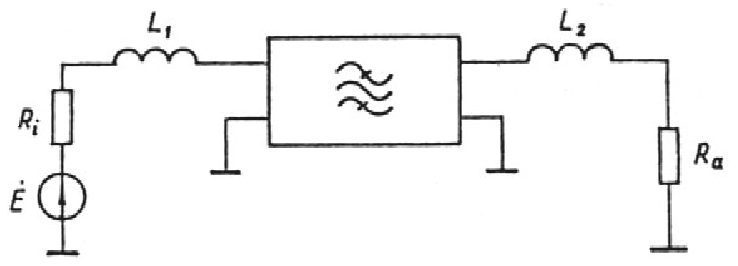
\includegraphics[width=400pt]{jungimo_schema.png}
\end{center}
\textsl{6.2 pav. Akustinio elektrinikos įtaiso jungimo schema.}\\

\begin{center}

\includegraphics[width=400pt,height=150pt]{keitiklio_eskizas.png}
\end{center}
\textsl{6.2 pav. Akustinio elektrinikos įtaiso keitiklio eskizas.}\\

Aptarta projektinių skaičiavimų metodika pagrįsta papraščiausiais keitiklių ir filtrų modeliais ir gali būti panaudojama 
orientaciniams skaičiavimams atlikti eskizinio projektavimo etape. Specialioje literatūroje galima rasti tobulesnius paviršinių 
akustinių bangų įtaisų modelius.

\section{Išvados}

Kursinio darbo metu ištyrėme terminės difuzijos procesą, kuris taikomas antrame silicion integrinių grandynų 
gamybos technologiniam procese, sudarėme tranzistorių ekvivalentinių grandinių schemas ir apskaičiavome jų parametrus. 
Suprojektavome akustoelektronikos įtaisą.\\

Ištyrę priemaišų pasiskirstymą po priemaišų įterpimo etapo iš grafiko galima pastebėti, jog, didinat proceso 
trukmę, galima padidinti priemaišos koncentraciją netoli bandinio paviršiaus. Iš priemaišos srauto tankio pokyčio, 
priemaišų įterpimo etape grafiko galima pamatyti, kad pradiniu laiko momentu priemaišos srauto tankio pokytis 
kinta tiesiškai priemaišos srauto tankio pokyčio didėjimo linkme ir didėjant laikui jis pradeda mažėti. Iš legiravimo 
dozės pokyčio, piemaišų įterpimo etape, grafiko galima pasakyti, jog kintant laikui legiravimo dozės pokytis didėje beveik tiesiškai 
didėjimo linkme. Nagrinėdami priemaišų pasiskirstymą po priemaišų perskirstymo etapo, didinant proceso trukmės laiką, 
galima sumažinti priemaišos koncentracija netoli paviršiaus staigiau. Iš priemaišos pasiskirstymas tranzistoriuje, 
formuoojamas dvikartės difuzijos būdu, grafiko galime pasakyti, kad netoli bandinio paviršiaus, priemaišos koncentracija 
kinta staigiaus mažėjimo kryptimi, paskui nežymiai pakyla ir likusio bandinio dalyje lieka pastovi.\\

Tirdami dvipolio tranzistorių, apskaičiavimo jo parametrus, sudarėme jo ekvivalentinę $\Pi$ pavidalo grandinę. 
Apskaičiavę $h$ parametrus, galime pamatyti, kad dvipolio tranzistoriaus įėjimo varža yra gan didelę ( $750 \Omega$ ), 
grįžtamojo ryšio koeficientas yra labai mažas ( šiuolaikiniuose tranzistoriuose jo visai nepaisoma ), srovės perdavimo 
koeficientas yra $181.25$, išėjimo laidumas yra $0.1mS$ arba išėjimo varža $10k \Omega$. Pasirinkę darbo tašką 
$K_{KQ} = 16.1 mA$ apskaičiavome tranzistoriaus perdavimo charakteristikos statumą $g_m$, kuris lygus 0.644. Žinodami 
$g_m$ ir $\beta$, kuri lygi bendro emiterio jungimo schemoje yra $h_{12E}$, apskaičiavome $r_{\pi}$, $r_0$ ir $r_{B}^{*}$. 
Žinodami vienetinio srovės perdavimo koeficiento dažnį, apskaičiavome tranzistoriaus parazitines talpas $C_{\pi}$.\\

Lauko tranzistoriaus perdavimo charakteristiką galima nubraižyti iš lauko tranzistoriaus išėjimo charakteristikos, pasirenkant 
$U_{SI}$ kaip konstantą ir keisdami $U_{UI}$, žiūrime kaip kinta $I_{S}$. Apskaičiavome lauko tanzistoriaus darbo taške 
$U_{UI} = 0.5 V$, $U_{SI} = 5 V$ perdavimo charakteristiko statumą, kuris lygūs santakos srovės ir užtūros-ištakos įtampos 
pokyčiui, ir tranzistoriaus išėjimo (vidinę) varžą, kuri lygi santakos-ištakos įtampos ir santakos srovės pokyčiui. Taip pat 
apskaičiavome tranzistoriaus dažnį, kuriam esant, tranzistorius nustoja stiprinti srovę $f_T = 159 Mhz$.\\

Projektuodami akustinį elektronikos įtaisą, pasitelkėme kompiuterinę programą, kuri mums pateikė tikslius akustinio 
elektronikos įtaisų parametrus, nubraižė įtaiso DACh. Iš skaičiavimu matome, kad akustoelektonikos įtaisas yra 
labai mažų gabaritų, tik 0.15 mm. Teoriniai filtrai nuo realių dažniausiai skiriasi dėl to, kad teoriniuose 
skaičiavimuose nebuvo atsižvelgta į aplinkos įtaką filtrui.\\

\section{Literatūra}

\begin{itemize}
	\item S.Štaras. Puslaidininkinės ir funkcinės Elektronikos įtaisai. Vilnius, "Technika", 2005, 468 p.
	\item S.Štaras. Elektronikos pagindai. Akustoelektronika. Vilnius, "TECHNIKA", 1994, 56 p.
	\item {\cyrrm{ Orlov V.S., Bondarenko V.S. "Fil{\cprime}try na poverchnostnykh akusticheskix volnakh", 1984 m. }}
\end{itemize}


\end{document}
